\documentclass[12pt]{article}

\usepackage{tikz}
\usetikzlibrary{mindmap}
\pagestyle{empty}

\begin{document}
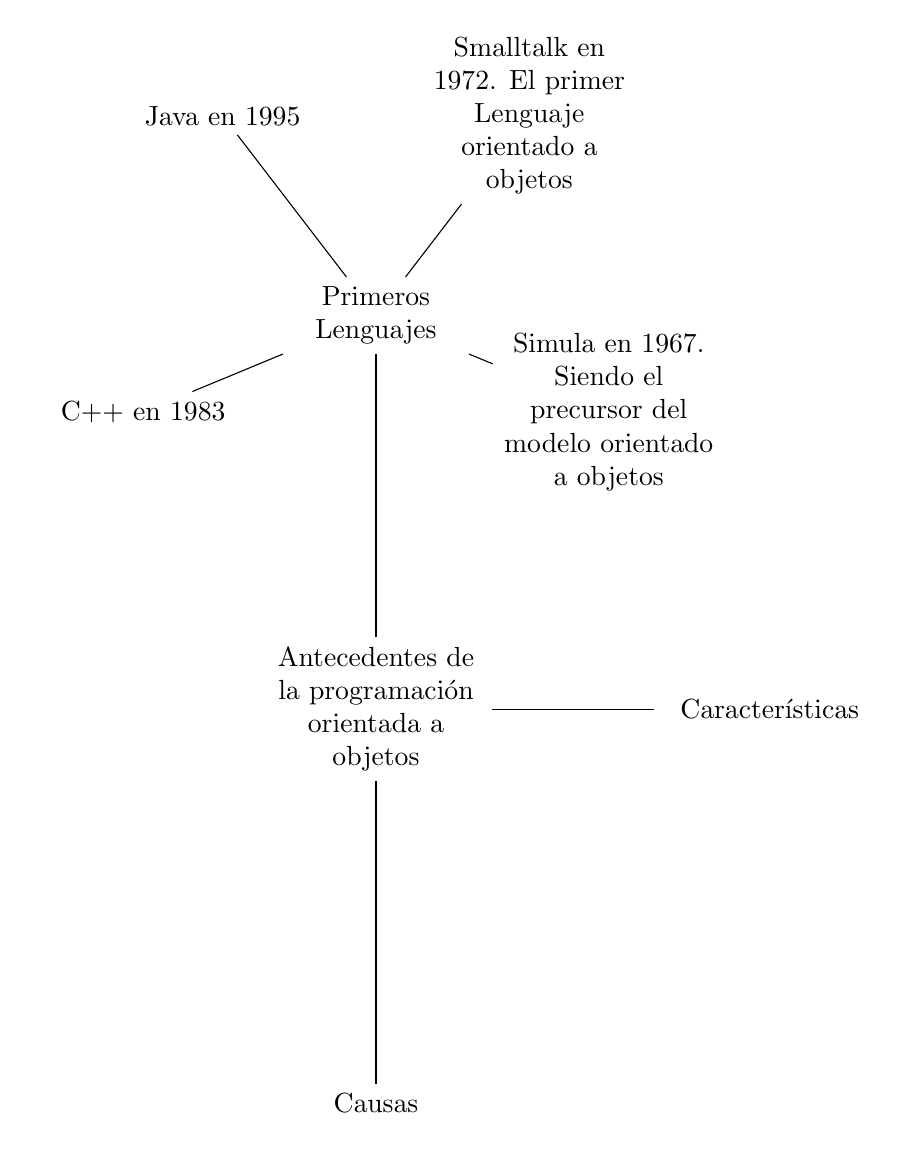
\begin{tikzpicture}[grow cyclic, text width=2.7cm, align=flush center,
        level 1/.style={level distance=5cm,sibling angle=90},
    	level 2/.style={level distance=3.2cm,sibling angle=75},
        level 3/.style={level distance=3cm,sibling angle=65}]]
    \node{Antecedentes de la programación orientada a objetos}
        child { node { Causas } }
        child { node { Características } }
        child { node { Primeros Lenguajes }
            child { node { Simula en 1967. Siendo el precursor del modelo orientado a objetos } }
            child { node { Smalltalk en 1972. El primer Lenguaje orientado a objetos } }
            child { node { Java en 1995 } }
            child { node { C++ en 1983 } }
        }
    ;
\end{tikzpicture}
\end{document}
